\chapter{Datamanagement}
\label{chap:datamanagement}
Deze lessen gaan over het importeren, opslaan, verwerken, en aanpassen van data voor later gebruik.

\section{Beheer van gegevens}
Of je nou analyses uitvoert, polymeren onderzoekt, nanotechnologisch bezig bent: als chemicus ben je constant bezig om data te verkrijgen, te verwerken, en te interpreteren. 

Een van de belangrijkste dingen hierbij is dat data systematisch wordt opgeslagen in een vorm die ook later nog bruikbaar is. De eerste les van dit onderdeel gaat hierover: welke technieken zijn er om je gegevens te beheren?

In dit onderdeel houden we het bij relatief simpele voorbeelden: gegevens die overzichtelijk in Excel-sheets passen en die door 1 persoon worden beheerd en gebruikt. Voor meer ingewikkelde gevallen heb je vaak databases nodig, om bijvoorbeeld grote hoeveelheden data te beheren of om meerdere personen op verschillende manieren toegang te kunnen verlenen. Databases komen aan bod in hoofdstuk~\ref{chap:gegevensbeheer}: Gegevensbeheer.

Voor het opslaan van data maak je van tevoren een plan, die je eventueel aanpast indien nodig. Het maken van een datamanagentsplan (DMP) is verplicht in veel sectoren: onderzoekers moeten bijvoorbeeld zo'n plan aanleveren bij de aanvraag van onderzoeksgeld. Er zijn een heleboel manieren om een dergelijk plan te maken. In dit hoofdstuk wordt er 1 manier doorgewerkt. Het is de bedoeling dat jullie ook een DMP maken voor jullie project Chemical Fingerprinting (en later ook voor Urban Mining).

Een datamanagementsplan bestaat uit verschillende aspecten. Hieronder worden de mogelijke onderdelen besproken, en er wordt meer informatie gegeven over technische aspecten. Vervolgens zal je een voorbeeldcase uitgewerken. In Appendix~\ref{ap:dmp} staat een sjabloon voor het maken van een DMP. 
\begin{itemize}
    \item \textbf{Algemene info}: Het plan bevat een voorblad met de meest essentiële informatie. Denk hierbij aan deelnemers (personen en organisaties), tijdsduur, datum, titel project, taken en rollen van personen
    \item \textbf{Verzamelen}: welk type data wordt er gegenereerd, hoe wordt deze verkregen, in welk formaat, de geschatte grootte van de dataset, de geschatte kosten, en of alles binnen wetgeving valt
    \item \textbf{Documentatie}: in welk format wordt de data opgeslagen, moeten er nog extra documenten bij met uitleg en metadata, in wat voor structuur wordt het opgeslagen, hoe wordt versiebeheer geregeld 
    \item \textbf{Opslag}: wat moet er allemaal worden opgeslagen, waar wordt het opgeslagen, wat zijn de kosten
    \item \textbf{Veiligheid}: is er betrouwbare data bij, wie mag bij welke data, moet data worden opgesplitst in losse sets, wie is de eigenaar van de data, en wat gebeurt er mee na het onderzoek
    \item \textbf{Selectie en behoud}: moet de data voor langere termijn worden bewaard, wie is daar verantwoordelijk voor, hoe wordt dat geregeld, hoe lang moet het worden bewaard
    \item \textbf{Reproductie}: wie mag de data verder gebruiken, welke licentie zit er op de data
\end{itemize}

De meeste onderdelen spreken voor zich. De technische aspecten zijn voor veel van jullie nog nieuw, dus daar wordt wat extra aandacht aan besteed.

\subsection*{Opslag van data}
Als je je bestanden wil opslaan zijn er een boel dingen waar je rekening mee moet houden. Ten eerste moet je weten in welk format je de data verkrijgt. Sommige meetapparaten geven de data in zogenaamde gepatenteerde bestandsformaten. Dit zijn bestanden die je niet zomaar kan openen in andere software. Als je dus je data opslaat op die manier is het mogelijk dat je later deze data niet meer kan openen. Het is dus zaak om te zorgen dat je data wordt opgeslagen op een manier zodat je er altijd bij kan. Bestandsformaten als .csv, .txt, .xlsx, .docx, .zip, zijn open bestandstypes die door erg veel verschillende software geopend kunnen worden. Bestandsformaten als .rar, .psd, .rtf, .wma, zijn gesloten bestandstypes die je alleen met specifieke software kan openen. Vaak is het noodzakelijk om de data van een meetapparaat te exporteren naar een open bestandstype. 

Naast het bestandsformaat is het ook erg handig om een begeleidend document bij de data te plaatsen die uitlegt wat de data precies is, wat de getallen voorstellen, etcetera. Dit wordt ook wel \textit{metadata} genoemd: data die wat zegt over andere data. Denk hierbij bijvoorbeeld aan een .txt bestandje die uitlegt in welke eenheid iedere kolom in een .xlsx bestand is opgeslagen.

Als de data is verzameld en is voorzien van metadata moet het worden opgeslagen. Een gebruikelijke manier is om dit te doen op een USB-stick. Dit is natuurlijk erg fout- en fraudegevoelig: de stick kan kwijtraken of kapotgaan, iedereen met de stick heeft toegang tot de data, er kan maar 1 persoon tegelijkertijd mee werken, etcetera. Dit is dus bijna nooit de goede manier om je data op te slaan.

Tegenwoordig is het bijna altijd standaard om de data op een server van het bedrijf/instelling op te slaan, of in een cloud-opslag zoals Dropbox, Google Drive, of OneDrive. Het is vaak zelfs verplicht om dit te doen om te zorgen dat de data ook voor andere onderzoekers beschikbaar en controleerbaar is, en zodat er automatisch back-ups worden gemaakt van het materiaal.

Hier moet je wel altijd goed nadenken over privacy en toegang. Als je bijvoorbeeld gevoelige informatie wil opslaan wil je niet dat iedere medewerker van je bedrijf daar bij kan, en als je samen wil werken met meerdere instellingen is het soms onmogelijk om dan alles op te slaan op een server van het bedrijf, aangezien niet iedereen daar toegang tot heeft.

In de regel sla je de data altijd op bij de cloud-opslag van je bedrijf, instelling, of school. In ons geval geldt dus dat je alles op gaat slaan op de OneDrive van het Saxion. Hiervoor moet je wel een goede mappen-structuur bedenken om de boel op te slaan: welke indeling wordt er gemaakt, welke bestanden komen erin, welke naamgeving hebben de bestanden, hoe wordt de metadata meegegeven, wie heeft toegang, etcetera. Dit hoort allemaal in je DMP terug te komen. 

\subsection*{Opdracht: Uitwerken datamanagementsplan}
\begin{figure}[h]
\begin{center}
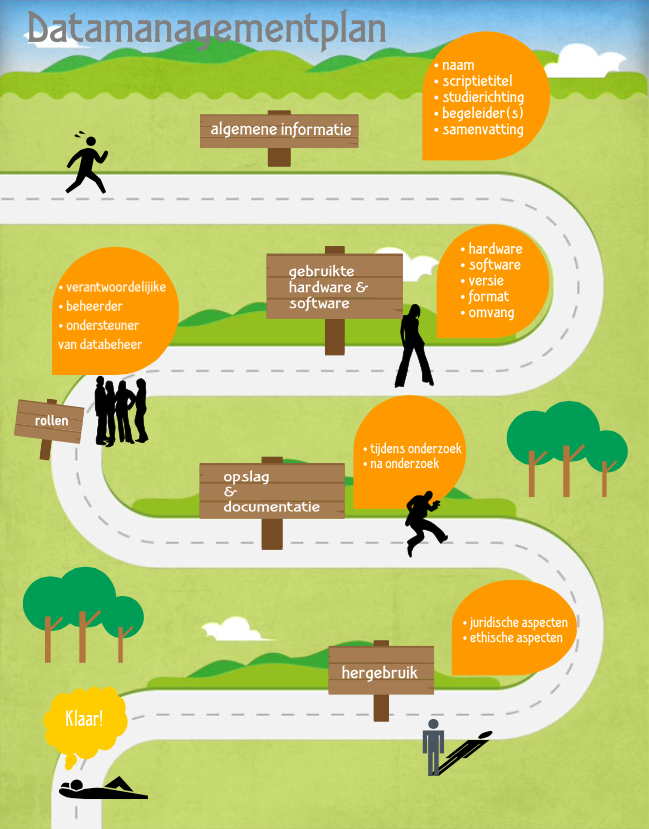
\includegraphics[width=0.6\textwidth]{img/dpm_studenten_infographic.png}
\caption{\label{fig:dmpinfo} \small Infographic voor het opstellen van een DMP. Gebaseerd op een werk van de Universiteitsbibliotheek Nijmegen op \href{http://ru.nl.libguides.com}{\textsf{http://ru.nl.libguides.com}}}
\end{center}
\end{figure}

In dit voorbeeld moet je een DMP opstellen voor een simpel onderzoek. In dit onderzoek worden fipronil-gehaltes bepaald in verschillende monsters. Fipronil is een schadelijke stof die een aantal jaren geleden in eieren terecht is gekomen, wat voor een landelijke herroeping van veel eieren heeft gezorgd. In dit onderzoek worden eieren van verschillende supermarkten onderzocht op fipronil-gehaltes. Het onderzoek wordt uitgevoerd bij het RIKILT (onderdeel van de Nederlandse voedsel- en warenautoriteit) door 2 studenten die daar stage lopen. 

Stap 1 in het DMP is het beschrijven van de algemene informatie:
\begin{table}[h]
\begin{tabular}{ll}
Onderzoekers    & H. van der Steeg, J. van der Maat                    \\
Titel onderzoek & Controleren van de gehaltes fipronil in supermarkteieren \\
Begeleiders     & Dr. B. Swennenhuis                                   \\
Bedrijf        & RIKILT Wageningen                                       \\
Datum      & 1/1/2020 tot 1/4/2020                                            
\end{tabular}
\end{table}

Nu moet er bedacht worden hoe de data wordt verkregen, opgeslagen, wie er verantwoordelijk is, etcetera.

\textbf{Details over het onderzoek}\\
Fipronil is een organisch molecuul wat wordt gemeten met behulp van een GC-MS. De ruwe data komt in .csv bestanden terecht en kan worden geanalyseerd met MSAnalyzer. De verwerkte data wordt opgeslagen als .xls bestand. De bestanden hebben een formaat van maximaal 1 MB per stuk (maar vaak een stuk kleiner). Er worden zo'n 100 eieren gemeten, en van ieder ei wordt zowel het eiwit als het eigeel doorgemeten in duplo. Alle ruwe data moet worden opgeslagen in verband met bewijslast. 

De MS wordt gebruikt om de fipronil-piek te identificeren en de hoogte van de piek in het chromatogram wordt gebruikt om het gehalte te bepalen. De uiteindelijk verwerkte uitkomsten van iedere meting (dus gehalte fipronil) zal in losse bestanden worden opgeslagen. 

De data wordt opgeslagen op de interne servers van het RIKILT. Hier kunnen alleen bevoegde medewerkers van het instituut bij. De bestanden moeten opgeslagen worden inclusief begeleidende tekst in het NL en EN die uitlegt wat er in de bestanden te vinden is en van welke sample de data afkomstig is. 

Er wordt verwacht dat de fipronilconcentratie onder de \SI[per-mode=symbol]{5}{\micro\gram\per\kilo\gram} ligt (maximaal toegestane waarde). Als de waardes hierboven liggen zal er direct melding van worden gemaakt bij de voedsel- en warenautoriteit in verband met een mogelijk gevaar voor de volksgezondheid. Bedrijven kunnen tot 5 jaar na overschrijding van maximale fipronilgehaltes een boete krijgen. 

\color{saxion}\textbf{Opdracht week 3: }\color{black} vul het sjabloon voor de DMP in voor deze case (zie appendix \ref{ap:dmp} of gebruik een ander sjabloon met een zelfde strekking), maak ook een voorbeeldmetadatabestand en mappenstructuur. Bewaar het gemaakte werk voor de eindopdracht.

\newpage
\section{Ordenen en opschonen van gegevens}
Als de gegevens uiteindelijk allemaal zijn verkregen is vaak de tweede stap om de data op te schonen, samen te voegen, en klaar te maken voor (semi-)langdurige opslag. Soms is dit heel simpel om te doen, maar vaak is dit een langduriger proces waarbij data uit verschillen bronnen en formats samengevoegd moeten worden tot een overzichtelijk geheel wat verder verwerkt kan worden.
Over het algemeen wordt hiervoor Excel gebruikt als softwarepakket. Met Excel kan je op veel verschillende manieren data importeren, inlezen, combineren, en weer opslaan in allerlei verschillende formats die door andere software kan worden ingelezen. In deze opleiding gebruiken we bijvoorbeeld R, SPSS, en Python om data verder te verwerken.

Let op: de screenshots van Excel die worden gegeven kunnen compleet verschillen van de versie van Excel die jij gebruikt. De functies zitten echter vaak op dezelfde plaats, maar werken soms wel net iets anders. Als je er niet uit komt: gebruik Google om handleidingen te zoeken. 

\subsection{Data importeren}

De data die je uit software verkrijgt kan in veel verschillende vormen worden aangeboden. Het kunnen .txt bestanden zijn, of .csv, of nog anders. Het handigste is om de data niet op te slaan in allerlei losse vormen, maar ze om te zetten naar 1 type bestand. Over het algemeen wordt data opgeslagen in .csv of .xlsx bestanden. Dit zijn namelijk bestandtypes die door de meeste software kan worden ingelezen voor verder gebruik.

.csv staat voor comma-separated-values, oftwel door komma gescheiden waardes. Dit zijn simpele bestanden in de vorm van text waarbij de data in kolommen staat, gescheiden door komma's (of soms tabs of spaties, maar dan is het eigenlijk geen .csv meer). Hieronder zie je een screenshot van een .csv bestand die geopend is in google sheets en in kladblok:

\begin{figure}[h]
\begin{center}
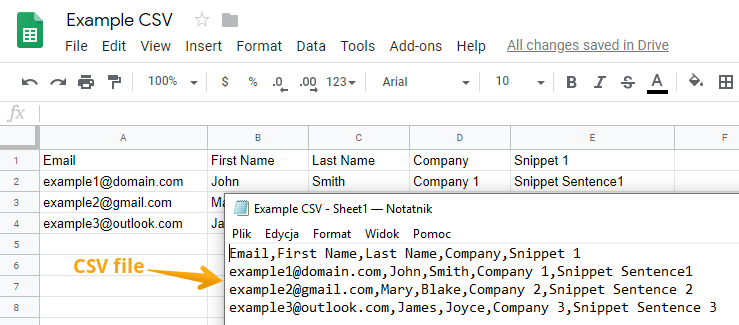
\includegraphics[width=\textwidth]{img/csv_ex.png}
\end{center}
\end{figure}

Zoals je ziet kan google sheets (of Excel) de data inlezen en laten zien in rijen en kolommen, en in klablok zie je per regel de waardes gescheiden van elkaar door komma's. Dit is exact dezelfde data, alleen op verschillende manieren weergegeven. 

Als je een .csv bestand opent in bepaalde software kan het zijn dat het direct wordt herkend en de data juist wordt weergegeven, maar soms is het bestand net iets anders opgemaakt, of herkent het programma het verkeerd. Daarom is het vaak nodig om de data te importeren in plaats van te openen. Hieronder wordt uitgelegd hoe je dat in Excel moet doen. Zodra je de data hebt geimporteerd kan je het bewerken, en opslaan als fatsoenlijk .csv bestand zodat je later er mee verder kan werken.

Over het algemeen kan je in het tabblad "Data" van Excel alle opties vinden voor het importeren van gegevens. In dit tabblad vind je (afhankelijk van je versie) verschillende manieren om data te importeren. Als je data vanuit een bestand wil inlezen selecteer je de optie "Get external data -> from text"

\begin{figure}[h]
\begin{center}
\includegraphics[width=0.5\textwidth]{img/Excelimport.png}
\end{center}
\end{figure}

Selecteer nu het bestand wat je wil importeren, en daarna kom je in de \textit{Import Wizard} terecht. Hierbij helpt Excel je de juiste opties te kiezen om de data te importeren. In het eerste scherm moet je kiezen of de data is gescheiden door tekens (bijvoorbeeld komma's, punten, puntkomma's, etc) of door spaties of tabs. In het scherm zie je onderin een voorbeeld van het bestand wat je wil importeren, kijk daar naar en kies de juiste optie. In het voorbeeld hieronder is de data gescheiden met puntkomma's, dus we kiezen de optie \textit{Delimited} (gescheiden door tekens, niet door spaties). Als je data ook een titel-regel heeft moet je dat ook in dit scherm aanvinken. 


\begin{figure}[h]
\begin{center}
\includegraphics[width=0.5\textwidth]{img/Excelimport2.png}
\end{center}
\end{figure}

Het kan ook zijn dat de data is gescheiden door komma's, maar de data ook zelf komma's bevat. Dan wordt er vaak gebruik gemaakt van aanhalingstekens om de data per cel duidelijk te krijgen, bijvoorbeeld in deze reeks waar met stapjes van een half wordt opgeteld:
\begin{verbatim}
    "0,0","0,5","1,0","1,5","2,0"
\end{verbatim}

In het volgende scherm moet je aangeven met welk teken de data is gescheiden. In dit geval zijn het puntkomma's, dus we vinken dat aan en we zien direct in het voorbeeld onderaan dat hij een streep zet tussen de twee kolommen. Als je deze streep niet ziet heeft Excel de scheiding niet goed herkend.

\begin{figure}[h]
\begin{center}
\includegraphics[width=0.5\textwidth]{img/Excelimport3.png}
\end{center}
\end{figure}

In het laatste scherm kan je kiezen wat voor type data het is: een getal, tekst, datums, etcetera. Dit is vaak erg belangrijk: Excel weet niet of een punt of een komma wordt gebruikt voor getallen, dat moet je bij het knopje "advanced" aangeven. Dit is iets wat vaak wordt vergeten en veel problemen oplevert! In NL wordt er een komma gebruikt als decimaal scheidingsteken, in de VS vaak een punt. Let hier dus goed op.

\begin{figure}[h]
\begin{center}
\includegraphics[width=0.5\textwidth]{img/Excelimport4.png}
\end{center}
\end{figure}

Vervolgens druk je op finish, kies je waar je de data wil hebben, en klaar. Controleer dat alle data goed is overgekomen en je hebt nu alles in je Excel-bestand staan!

\color{saxion}\textbf{Oefenopdracht: }\color{black} ga naar \href{https://people.sc.fsu.edu/~jburkardt/data/csv/csv.html}{\textsf{https://people.sc.fsu.edu/$\sim$jburkardt/data/csv/csv.html}}, download minimaal 3 .csv bestanden en importeer deze in Excel. Sla op als .xlsx bestand met 3 tabbladen die de data bevatten uit de drie .csv's.

\subsection{Data bewerken en rangschikken in Excel}
Zodra je de data netjes in een .xlsx of .csv bestand hebt kan je het opslaan, maar als je er verder mee wil werken moet er vaak nog aan gesleuteld worden: slechte waardes moeten eruit, opmaak bij de tabellen, eventueel grafieken, samenvoegen van datasets, etcetera. In dit deel worden er aan de hand van een voorbeeld verschillende bewerkingen in Excel tentoongesteld.

In dit voorbeeld gebruiken we een dataset van wijn-gegevens. Deze dataset bestaat uit twee bestanden, met iedere meerdere kolommen, waarbij iedere wijn is doorgemeten op verschillende wijzes in veelvoud. De details worden achterwege gelaten, die zijn niet relevant voor het voorbeeld. 

\subsubsection*{Tabel maken}
Over het algemeen hou je de data zo kaal mogelijk, zodat je het makkelijk kan importeren en exporteren. Als je de data netjes wil presenteren, of je wil het wat overzichtelijker maken: Excel kan ook gebruikt worden om nette tabellen te maken.
In eerste instantie ziet de dataset er zo uit (.csv bestand):

\begin{figure}[h]
\begin{center}
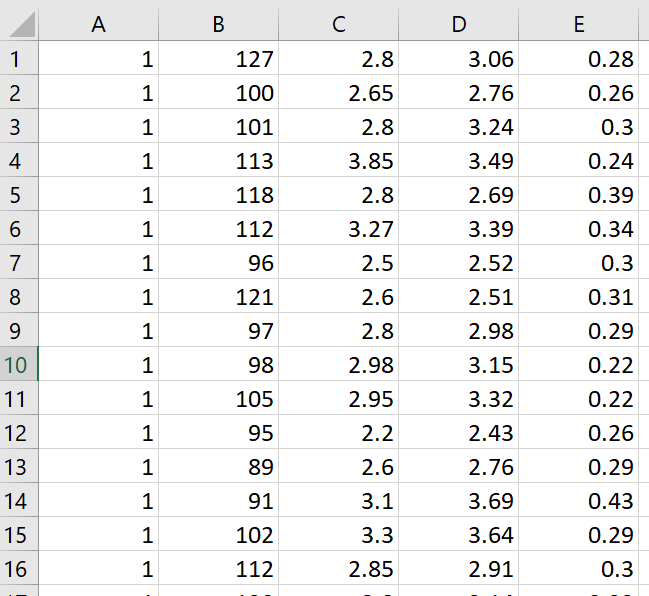
\includegraphics[width=0.5\textwidth]{img/wijn1.png}
\end{center}
\end{figure}

Het is vaak handig om een titelregel toe te voegen. Dit doe je door rechtermuisklik -> insert te klikken op de bovenste regel.

\begin{figure}[h]
\begin{center}
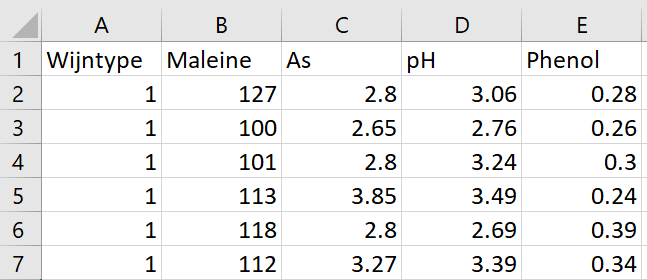
\includegraphics[width=0.5\textwidth]{img/wijn2.png}
\end{center}
\end{figure}

Als je het netjes wil opmaken en bruikbaar wil maken voor mensen maak je de datasheet op als tabel. Selecteer de data en druk (rechtsboven) op de knop "Format as Table". Kies een kleur en druk op OK om de tabel te maken.
\begin{figure}[h]
\begin{center}
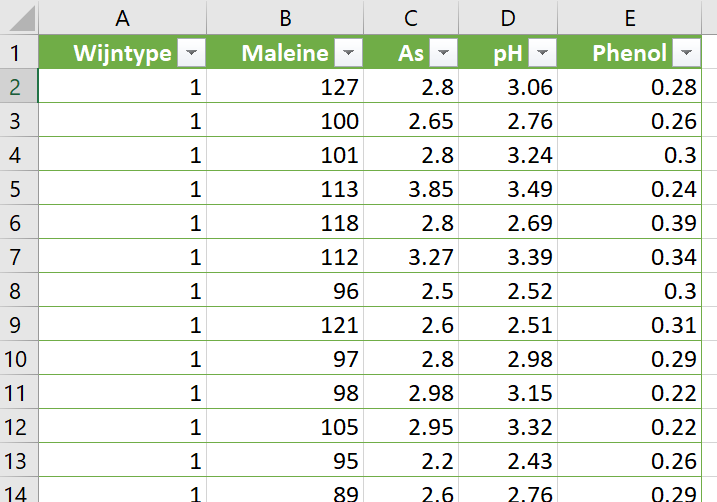
\includegraphics[width=0.5\textwidth]{img/wijn3.png}
\end{center}
\end{figure}

Je ziet nu ook pijltjes bij de vakjes op de bovenste regel: dit kan je gebruiken om bv te sorteren en zoeken in de tabel. Dit kan erg handig zijn! Klik hier een keer rond en bekijk de opties.

Er is nog een ander voordeel om je data als tabel in te delen: het verwijzen naar data in formules gaat een stuk eenvoudiger met tabellen ten opzichte van 'kale' data. Als je bijvoorbeeld naar een kolom met data wil verwijzen gebruik je normaal in excel iets als dit:
\begin{verbatim}
    C1:C14
\end{verbatim}

Als je een tabel hebt met titels, zoals in het voorbeeld de kolom As van tabel Wijn kan je ook zo verwijzen:

\begin{verbatim}
    Wijn[As]
\end{verbatim}

Dat is een stuk beter leesbaar, en als je meer regels aan je tabel toevoegt hoef je de verwijzing niet aan te passen. Bij het gebruik van Tabellen zal Excel automatisch de meest handige manier van verwijzen gebruiken.

Sla het bestand uiteindelijk opnieuw op als .xlsx bestand. Als het een .csv bestand blijft kan je veel opties niet gebruiken, en je wil je .csv bestand kaal houden als ruwe data. 

\subsubsection*{Berekeningen}
In Excel kan je uiteraard van alles berekenen. Er zijn een heleboel functies beschikbaar om dat voor je te doen. De basis wordt hier uitgelegd, en als je meer of andere bewerkingen wil doen moet je zelf zoeken op het internet.

Om een berekening uit te voeren typ je in een lege cel een = teken, met daarachter je berekening. Bijvoorbeeld als je cel A2 en B2 bij elkaar wil optellen:

\begin{verbatim}
    =A2+B2
\end{verbatim}

Naast simpele operaties zijn er ook functies die je kan uitvoeren. Om een of andere reden heeft Microsoft besloten dat deze functies in verschillende talen anders heten, wat erg storend is. In dit dictaat wordt het in het Engels weergegeven, maar als je je computer in het Nederlands gebruikt moet je dus andere functies intypen voor hetzelfde effect. Online kan je de 'vertalingen' vinden. 

Een voorbeeld van een functie is bijvoorbeeld AVERAGE die het gemiddelde uitrekent van een reeks, bijvoorbeeld:
\begin{verbatim}
    =AVERAGE(A1:A24)
    =AVERAGE(A:A)
    =AVERAGE(A1:D30)
\end{verbatim}
Waarbij de eerste regel het gemiddelde van cel A1 t/m A24 uitrekent, de tweede regel het gemiddelde van alle A-cellen, en de laatste regel A1-30, B1-30, C1-30 en D1-30 allemaal uitmiddelt. 

Als je een functie hebt ingevoerd kan je die ook doortrekken naar meerdere cellen, als je bijvoorbeeld het gemiddelde van iedere rij wil weten. Excel past vaak zelf de cellen aan zodat er een logisch antwoord uitkomt. Als je een functie wil kopieren maar je wil dat de verwezen cellen niet veranderen kan je het dollarteken gebruiken zoals hier:
\begin{verbatim}
    =AVERAGE($D4)
    =AVERAGE(D$4)
    =AVERAGE($D$4)
\end{verbatim}
Waarbij in de eerste regel de letter vast staat, in de tweede regel het cijfer, en in de derde regel beiden.

Er zijn uiteraard nog veel meer functies, en ook veel complexere functies. Over het algemeen adviseren we het meer ingewikkelde werk niet in Excel te doen maar in software als R of Python. Dat komt volgend kwartiel onder andere aan bod. Hieronder een paar functies die handig zijn om te kennen. Probeer ze zelf ook uit in een datasheet van jezelf!

\begin{verbatim}
    =COUNTIF(A1:A30, ">5")
    telt tussen A1 en A30 hoeveel vakjes boven de 5 zijn
    
    =AVERAGEIF(A1:A30, ">3")
    =SUMIF(A1:A30, "<1")
    zelfde maar met optellen/gemiddelde
    
    =MAX(A1:A30)
    =MIN(A1:A30)
    geeft de hoogste/laagste waarde in gebied
    
    =IF(A1>5,"Hoog","Laag")
    Checkt voorwaarde (a1>5), als dat is dan komt "hoog"
    in het vakje, anders komt "laag" in het vakje.
\end{verbatim}

Je kan deze functies ook combineren, uitbreiden, etcetera. Met een beetje hulp van Google en proberen kom je vaak een heel eind. 

\subsubsection*{Samenvoegen}
Het komt ook vaak voor dat je data verspreid over meerdere datasets staat, maar dat je dat graag in 1 overzicht wil hebben. Hier is natuurlijk ook een functie voor. In principe zijn er 3 manieren om dit te doen: Met de hand (vaak te veel werk en onhandig), met VLOOKUP, of met INDEX en MATCH. VLOOKUP wordt hier niet behandeld omdat dat traag en niet flexibel is, dus we gebruiken hier eigenlijk altijd INDEX en MATCH voor. Als je Excel in het Nederlands gebruikt is het geen INDEX en MATCH, maar INDEX en VERGELIJKEN. Aan de hand van een voorbeeld worden deze functies hier uitgelegd.


\begin{figure}[h]
    \centering
    \begin{minipage}{0.45\textwidth}
        \centering
        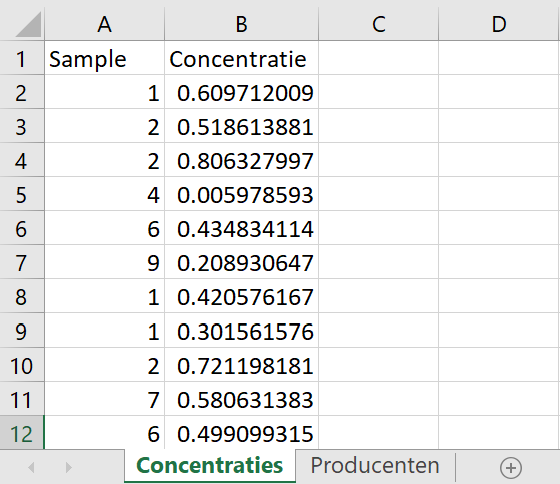
\includegraphics[width=0.9\textwidth]{img/index1.png} 
    \end{minipage}\hfill
    \begin{minipage}{0.45\textwidth}
        \centering
        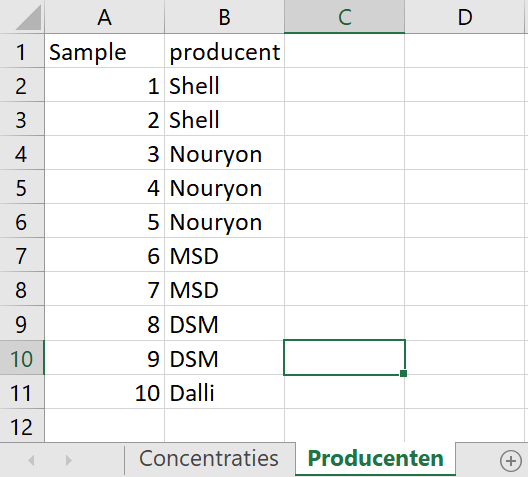
\includegraphics[width=0.9\textwidth]{img/index2.png}
    \end{minipage}
\end{figure}

In dit voorbeeld worden samples van verschillende producenten doorgemeten. De analist krijgt een sample met een nummer en meet de concentratie. Later wordt er opgezocht van welke producent welke sample is. We hebben nu dus een Excel-bestand met twee tabbladen: eentje met de gemeten concentraties en eentje met de producent per sample.

We willen nu graag in tabblad 1 (concentraties) een nieuwe kolom toevoegen waar de producent van de sample staat die erbij hoort. Dit doen we met index en match. In de derde kolom (C) vullen we de volgende code in op C2 en trekken dit door naar de rest van de tabel:
\begin{verbatim}
=INDEX(Producenten!$B$2:$B$11,MATCH(Concentraties!A2,Producenten!$A$2:$A$11,0))
\end{verbatim}
\begin{figure}[h]
\begin{center}
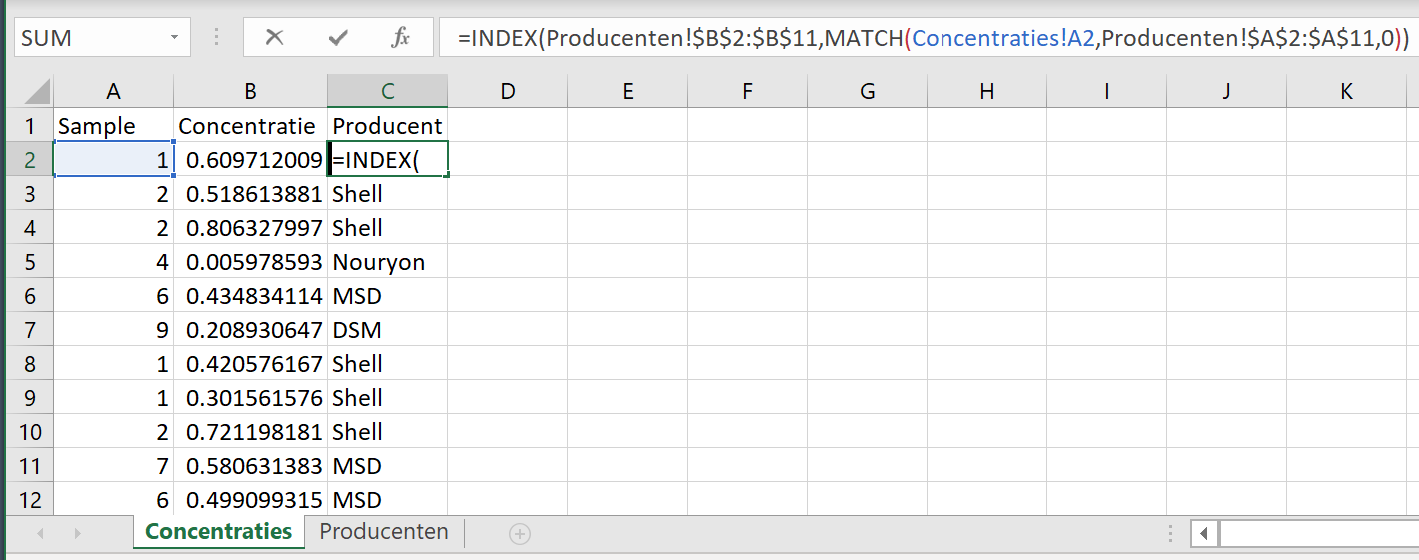
\includegraphics[width=0.9\textwidth]{img/index3.png}
\end{center}
\end{figure}

Zoals je ziet staan nu de juiste namen naast de samples. Er wordt nu stuk voor stuk uitgelegd wat je waar in moet vullen. Er zijn 4 dingen om in te vullen in de functie:

\begin{verbatim}
    =INDEX(bron, MATCH(item, lijst, 0))
\end{verbatim}
Van links naar rechts gaan we langs de losse parameters. "bron" is de kolom waar de gegevens instaan die je uiteindelijk wil hebben. In dit geval willen we de naam van de producent hebben, dus geven we aan waar we \textit{alle} namen van producenten kunnen vinden: in kolom B van tabblad Producenten. Dat geven we aan in Excel met \textsf{Producenten!B2:B11}, en er zijn dollartekens toegevoegd om het constant te houden. 

De volgende parameter die we moeten opgeven is \textit{item}. Hier vullen we in welk item we opzoeken: dit moet dus iets zijn wat in beide tabbladen aanwezig is. In dit geval is dat het samplenummer. We gebruiken dus het samplenummer van het tabblad concentraties: dat is het sample wat bij die regel hoort en die vinden we in kolom A (en in dit geval op regel 2) op het tabblad Concentraties: Concentraties!A2.

Nu moeten we aangeven waar de lijst met samplenummers is in het tabblad producenten: dat is ook kolom A. We geven dus aan Producenten!A2:A11. 

Tot slot moet je nog een 0 toevoegen. Dit zorgt ervoor dat Excel alleen exacte matches teruggeeft. Dit wil je eigenlijk altijd. 

Als je meer voorbeelden wil kan je die online vinden, bijvoorbeeld hier:\\
\href{https://www.deskbright.com/Excel/using-index-match/}{\textsf{https://www.deskbright.com/Excel/using-index-match/}}. 

Het is bijna zeker dat je deze functie nodig hebt bij het project Chemical Fingerprinting, aangezien je dezelfde sample gaat meten met verschillende apparaten. Hou de ruwe data apart, en gebruik INDEX en MATCH om een overzichtsbestand te maken.

\color{saxion}\textbf{Oefenopdracht: }\color{black} Ga naar Blackboard en download Pottery.csv en Pottery2.csv. Gebruik Excel om de data samen te voegen op 1 pagina (met index en match) en een nette tabel te maken van de data met op 1 tabblad:
\begin{itemize}
    \item Geformatteerd als tabel
    \item Een extra kolom met daarin het gemiddelde van iedere regel
    \item Een extra regel met daarin de hoogste waarde van iedere kolom
    \item Een los vakje met daarin de hoogste Al-waarde van de hele tabel, met daarnaast het nummer van het sample wat daarbij hoort
    \item Een extra kolom die aangeeft per regel of er waardes onder de 0.05 in de regel zit met "Ja" of "Nee". Bonus: gebruik "conditional formatting" om alle vakjes met Ja rood te kleuren.
    \item Een los vakje met daarin het aantal meetwaardes boven de 1
    \item Een los vakje met daarin het aantal samples
\end{itemize}

Het excelbestand zou er uiteindelijk ruwweg zo uit moeten zien:
\begin{figure}[h]
\begin{center}
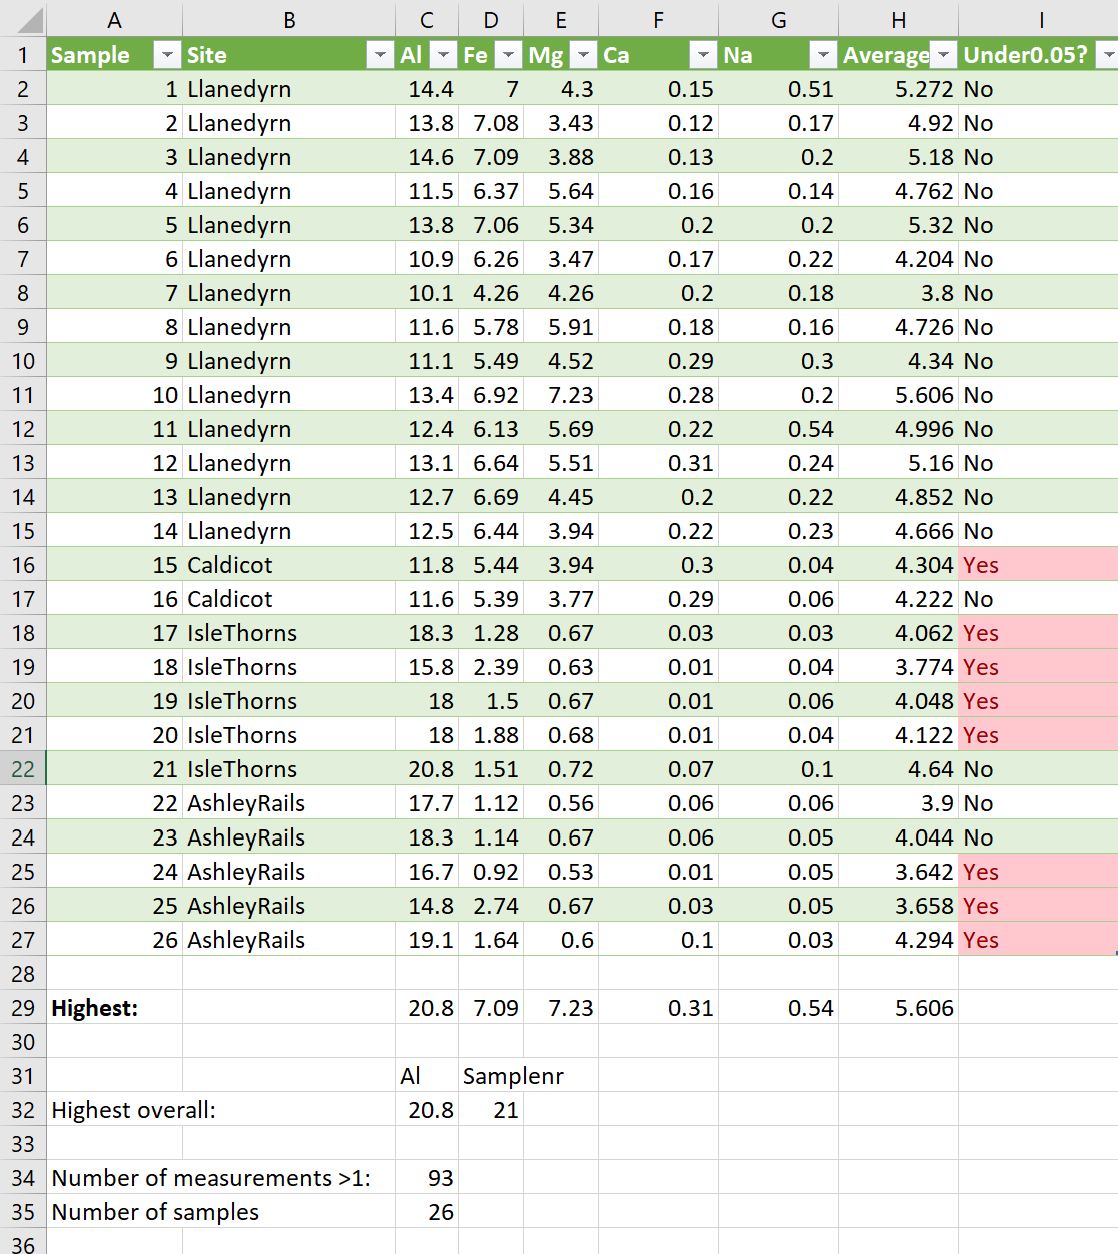
\includegraphics[width=0.4\textwidth]{img/xlsx.png}
\end{center}
\end{figure}
\\
\color{saxion}\textbf{Eindopdracht week 4: }\color{black} Gebruik de kennis die je hebt vergaard de afgelopen 2 weken om een DMP te schrijven (en uit te voeren!) voor het project Chemical Fingerprinting. De data die je verzamelt voor het project ga je volgend kwartiel gebruiken voor een automatiseringsopdracht, dus het is van belang dat je de data op een goede manier opslaat! Neem dus ook in je plan op hoe je data van de meetapparatuur gaat inlezen, omzetten en op gaat slaan. Leg dus ook uit welke Excel-bewerkingen je gaat doen om je data te rangschikken, presenteren, enzovoorts. 